\chapter{Thermal Hydraulics}
\label{ch:thermalHydraulics}

\section{Introduction}
  For reactor design purposes, designs are ultimately constrained by thermal
  properties. Additionally, neutronics properties in the form of cross sections
  and density changes are significantly affected by system temperatures.
  Therefore, to accurately simulate the neutron distribution within the reactor,
  it is necessary to also simulate temperatures within the reactor.

  In this simulation, two thermal hydraulic models are
  employed. The first is a one-dimensional fluid flow model to calculate coolant
  temperatures as the coolant flows through a channel. This model is valid for
  the assumption of no cross-flow between channels and perfect fluid mixing 
  within the flow channel. For use in simulating fast reactors with canned
  assemblies and assembly designs which encourage mixing, these assumptions are
  valid. The second model used is a radial
  pin-conduction model to calculate cladding, sodium bond, and fuel temperatures
  based on the heat conduction equation.

  For the purposes of the thermal hydraulics model, geometry is described in
  \fref{fig:radial_model}. This model represents a cylindrical fuel pellet,
  surrounded by sodium bond, enclosed in steel cladding, with sodium coolant
  flowing in the axial direction. The center of the fuel pin is located at
  $r=0$ where $r$ is the radial coordinate. The fuel pellet has radius $R_F$ and
  fuel is located in $r \in [0,R_F)$. Then, bond is located in $r \in (R_F,R_B)$
  and clad is located in $r \in (R_B,R_C]$. The fuel center-line temperature is
  $T_0$ and fuel surface temperature is $T_F$. Bond surface temperature is
  $T_B$ and clad surface temperature is $T_C$. $T_{\infty}$ represents the bulk
  coolant temperature. In this model, heat is generated exclusively in the fuel
  with volumetric heat generation rate $q'''$. 
  
  \begin{figure}
    \centering
    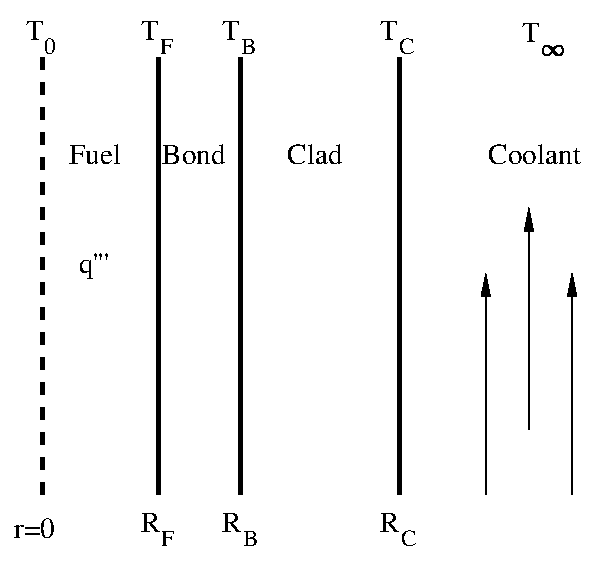
\includegraphics[width=0.5\textwidth]{radial_model}
    \caption{Geometry Description for Thermal Hydraulics Model.}
    \label{fig:radial_model}
  \end{figure}

  Used in association with an unstructured mesh, the thermal hydraulic model
  requires mapping mesh elements to flow channels. In the user input to the
  program, the user must specify to which one-dimensional flow channel belongs.
  Adopting the nomenclature from fast reactors, each flow channel represents a
  hexagonal-assembly or a ``hex''. In the following discussion, a hex index is
  subscripted $h$ for $h = 1,2,\ldots,N_h$ where $N_h$ is the number of
  hexagonal assemblies in a reactor. Though the term ``hex'' is used, there is
  no assumption made in any of the calculations that the assembly is indeed
  hexagonal. Square one-dimensional assemblies would be simulated similarly.

  The user must specify $Q_{Rx}$ as the total heat output by the reactor and
  $\mdot_{Rx}$ as the total coolant mass flow into the reactor. Mass flow is
  then partitioned into each channel assuming constant mass flux at the reactor
  inlet. That is, the mass flow per unit area is assumed constant at the reactor
  inlet and the mass flow in a channel is the product of the mass flux and the
  channel flow area. The user must also input $T_{inlet}$ as the temperature at
  the inlet to the reactor.

  The concept of ``chunks'' is also introduced to aid in the discretization of
  the thermal hydraulic model. A chunk is the set of all elements in a channel
  with a unique axial elevation. For example, in a fast reactor hexagonal
  assembly, the assembly has a unique $h$ index and contains a number of chunks
  equal to the number of axial elevations in the simulation. Additionally, each 
  chunk is required to have unique material composition. The concept of chunks
  is shown in \fref{fig:chunk_description}.  Chunks are indexed
  $c = 1,2,\ldots,N_c$ where $N_c$ is the total number of chunks. For $N_z$
  axial elevations, $N_c = N_h \, N_z$. The indexing
  of chunks is chosen such that $c+N_h$ is the chunk one axial elevation above
  chunk $c$. 

  \begin{figure}
    \centering
    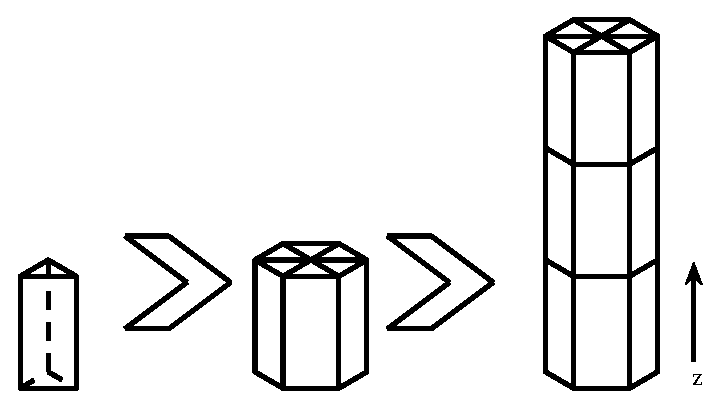
\includegraphics[width=0.7\textwidth]{chunk_description}
    \caption{Progression of Element (left), to Chunk (center), to Hex (right).}
    \label{fig:chunk_description}
  \end{figure}

\section{Power Calculation}
  Recall the multigroup neutron diffusion equation solved via the power
  iteration method returns the largest eigenvalue $\keff$ and unique positive
  eigenvector $\phi_g$ (see \sref{sec:power_iterations}). The flux calculated
  according to this method can be normalized to an arbitrary constant. For a
  specified value $Q_{Rx}$ the normalization constant can be calculated. For
  un-normalized neutron flux $\widetilde{\phi_{g,e}}$ with group $g$ in element
  $e$, the normalization constant is written as
  \begin{equation}
    \label{eq:normalization_c}
    c = \frac{Q_{Rx}}{\sum_{g}^{G} \sum_{e}^{N_E} \kappa \Sigma_{f,g,e} \,
      \widetilde{\phi_{g,e}}}
  \end{equation}
  where $c$ is the normalization constant. $\kappa$ represents the reclaimable
  (non-neutrino) energy produced per fission such that the quantity $\kappa
  \Sigma_f \phi$ represents the heat generation rate. Then the true reactor
  neutron flux is given as
  \begin{equation}
    \label{eq:normalization_phi}
    \phi_{g,e} = c \, \widetilde{\phi_{g,e}}
  \end{equation}
  and the power distribution is 
  \begin{equation}
    \label{eq:normalization_q}
    q_{e} = \sum_g^G \kappa \Sigma_{f,e,g} \phi_{g,e}.
  \end{equation}
  For an elemental power $q_e$, then the volumetric heat generation rate within
  the fuel is 
  \begin{equation}
    \label{eq:elementqppp_fuel}
    q'''_{e} = \frac{q_e}{V_{fuel,e}}
  \end{equation}
  where $V_{fuel,e}$ is the volume of fuel in element $e$. This will be
  necessary for the radial conduction model.

  For the one-dimensional heat convection model in the axial direction,
  heat generation quantities are needed for chunks instead of elements.
  The quantities required are then the total heat generated in a chunk $q_c$ and
  the average volumetric heat generation rate in the fuel for elements within
  the chunk $q'''_c$. These relationships are given in \eref{eq:chunkpwr} and
  \eref{eq:chunkqppp_fuel} respectively. The notation $e \in c$ implies the
  summation over all elements $e$ within chunk $c$.
  \begin{align}
    \label{eq:chunkpwr}
    q_c = \sum_{e \in c} q_e \\
    \label{eq:chunkqppp_fuel}
    q'''_c = \frac{\sum_{e \in c} q'''_e V_{fuel,e}}{\sum_{e \in c} V_{fuel,e}}
  \end{align}

\section{Axial Convection Model}
  The coolant enthalpy for an axial location $z$ within the channel is expressed
  by a simple heat balance equation as
  \begin{equation}
    \label{eq:continuous_heat_balance}
    h_h(x) = h_{in} + \frac{1}{\mdot_h} \int_0^z q'_h(z') \; dz'
  \end{equation}
  where $h$ is the specific enthalpy, $h_{in}$ is the inlet enthalpy, $\mdot_h$
  is the mass flow rate within the channel, and $q'_h(x)$ is the linear heat 
  generation rate for channel $h$ at elevation $z$. $h_{in}$ is related to
  $T_{inlet}$ by a state relationship for the coolant. The integral in
  \eref{eq:continuous_heat_balance} can be discretized along the channel and
  converted to a summation.
  \begin{equation}
    \label{eq:heat_balance}
    h_c = h_{in} + \frac{1}{\mdot_h} \sum_{i}^{N_z} q'_{i,h} \Delta z_{i,h}
  \end{equation}
  where $q'_{i,h}$ is the linear heat generation rate at axial level $i$ in 
  channel $h$ and $\Delta z_{i,h} = z_{i+1,h} - z_{i,h}$. (Note: by indexing
  properly, $c = h + (i-1) \, N_h$.) Recognizing the 
  quantity $q'_{i,h} \Delta z_{i,h}$ is the total heat generated in channel $h$ 
  at axial level $h$, then \eref{eq:heat_balance} can be rewritten.
  \begin{equation}
    h_c = h_{in} + \frac{1}{\mdot_h} \sum_i^{N_z} q_{i,h}
  \end{equation}
  
\section{Radial Conduction Model}
  \subsection{Derivation}
  \subsection{Relations}
\section{Cross Section Treatment}
  \subsection{Cross Section Library Generation}
  \subsection{Temperature Dependent Cross Section Calculation}

% todo this will probably be a separate chapter and include thermal expansion
%\section{Results}
%  \subsection{Single Pin Model}
%  \subsection{Reactor Simulation}
